% !TeX encoding = UTF-8
% !TeX spellcheck = en_US
\documentclass[a4paper,DIV=12,BCOR=1cm,
	twoside,toc=listofnumbered,bibliography=totocnumbered,numbers=noenddot]{scrreprt}
	\usepackage[utf8]{inputenc} % Sonderzeichen
	\usepackage{fancyhdr} % Kopf-, Fußzeilen
	\usepackage{graphicx} % Bilder	
	\usepackage[bookmarksopen,
				bookmarksopenlevel=0,
				pdfborder={0 0 0}]{hyperref} % Hyperlinks
	\usepackage{amsmath} % Mathe, lädt amsmath gleich mit
	\usepackage{amssymb} % Mathesymbole
	\usepackage{paralist} % Nummerierungen a) etc. von Umgebungen
	\usepackage{todonotes}

	% numbering for figures, footnotes and tables not chapter-based
	\usepackage{chngcntr}
	\counterwithout{figure}{chapter}
	\counterwithout{footnote}{chapter}
	\counterwithout{table}{chapter}

	% gantt diagrams
	\usepackage{pgfgantt}

	% Import title etc. constants
	% !TeX spellcheck = en_US
\def\Author{Patrick Robrecht}
\def\ThesisType{Master's Thesis}
\def\Title{Incremental Unidirectional Model Transformation via Graph Transformation with eMoflon::IBeX}
\def\Keywords{graph transformation, graph transformation tool, eMoflon, model transformation, unidirectional model transformation, model modification}

\def\Supervisor{Jun.-Prof. Dr. Anthony Anjorin}
\def\SecondExaminer{Prof. Dr. Gregor Engels}
\def\DateOfProposalSubmission{March 8, 2018}
\def\DateOfThesisSubmission{July 12, 2018}

\def\ResearchGroup{Database and Information Systems}
\def\Address{Fürstenallee 11, 33102 Paderborn}

% own commands
\newcommand{\eg}{e.\,g. }
\newcommand{\ie}{i.\,e. }
\newcommand{\create}{{\color[rgb]{0,0.5,0} \texttt{++}}}
\newcommand{\delete}{{\color[rgb]{1,0,0} \texttt{--}}}

% common includes
\usepackage{tikz}
\usetikzlibrary{
	arrows,
	calc,
	positioning
}

% (class diagrams)
\usepackage{../../master-thesis-gt-tool/common/tikz-uml}
\tikzset{
	class/.style = {
		inner sep = 0
	}
}
\newcommand{\methodSep}{\\[-4px]}

% tables
\renewcommand{\arraystretch}{1.5}
\usepackage{longtable} % allows to use footnotes in table
\usepackage{booktabs}
\usepackage{pifont}
\newcommand{\yes}{{\color{green}$\checkmark$}}
\newcommand{\no}{{\color{red}\text{\ding{55}}}}

% listings
\definecolor{commentcolor}{rgb}{0,0.4,0.2}
\definecolor{keywordcolor}{rgb}{0.50,0.00,0.33}

\usepackage{listings}
\lstset{
	aboveskip = 15pt,
	basicstyle = \small\ttfamily,
	breaklines = true,
	captionpos = b,
	commentstyle = \color{commentcolor},
	emphstyle = \bfseries,
	numbers = left,
	numbersep = 10pt,
	numberstyle = \scriptsize \color{gray},
	keywordstyle = \color{keywordcolor},
	language = Java,
	tabsize = 4,
	xleftmargin = 20pt,
	frame = lrtb,
	framexbottommargin = 5pt,
	framexleftmargin = 20pt,
	framexrightmargin = 5pt,
	framextopmargin = 5pt
}

	
	\hypersetup{
		pdftitle = {\Title},
		pdfsubject = {\ThesisType~Proposal},
		pdfauthor = {\Author},
		pdfkeywords = {\Keywords},
	}

% Title Settings
	\title{\ThesisType~Proposal: \Title}
	\author{\Author}
	\date{\DateOfProposalSubmission}


\begin{document}
	\addtolength{\oddsidemargin}{0.75cm}
	\begin{titlepage}
		\begin{center}
			\begin{minipage}{13.5cm}		
				\includegraphics[height = 2.4cm]{../common/figures/university-logo-en} \\[3pt]
				\textsf{
					\hspace*{2.2cm} Faculty for Computer Science, Electrical Engineering and Mathematics \\
					\hspace*{2.2cm} Department of Computer Science \\
					\hspace*{2.2cm} \ResearchGroup \\
					\hspace*{2.2cm} \Address
				}
			\end{minipage}\\[60pt]
			
			{\Huge\bfseries
				Incremental Unidirectional \\
				Model Transformations \\
				via Graph Transformation \\[5pt]
				with eMoflon::IBeX} \\[30pt]
			
			{\LARGE \ThesisType~Proposal} \\[30pt]
			
			by \\[5pt]
			
			{\scshape\large \Author} \\[30pt]
			
			submitted to \\[5pt]
			
			{\scshape\large \Supervisor} \\[5pt]
			
			and \\[5pt]
			
			{\scshape\large \SecondExaminer} \\[40pt]
			
			{Paderborn, \DateOfProposalSubmission}
		\end{center}
	\end{titlepage}
	\addtolength{\oddsidemargin}{-0.75cm}
	
	% header and footer
	\newcommand{\fancy}{
		\fancyhf{}
		\renewcommand{\headrulewidth}{0.0pt}
		\fancyfoot[C]{}
		\fancyfoot[LO,RE]{\scriptsize \Author: \Title ~(Proposal)}
		\fancyfoot[LE,RO]{\small \thepage}
		\renewcommand{\footrulewidth}{0.5pt}
	}	
	\pagestyle{fancy}
	\fancy
	\fancypagestyle{plain}{\fancy}


	\pdfbookmark[1]{Table of Contents}{toc}
	\tableofcontents

	\renewcommand{\clearpage}{}
	\newpage

	% !TeX spellcheck = en_US
\chapter{Introduction}
\label{introduction}

\textit{Model-driven engineering} (MDE) is an approach in software development which focuses on the specification of software artifacts in the application domain.
It raises the abstraction level from programming to domain-specific modeling languages by the use of \textit{models} for the representation of knowledge.
The MDE approach aims for a simplification of the specification process and improvement of the communication between different people and teams working on a system (cf. \cite{MDEVoelter}, p. 13; \cite{HerringMernikWhenAndHowDevelopDSLs}).

\textit{Model transformations} can be used to transform models into other models, \eg modifying an existing model or generating code from a model.
Other application areas are web applications \cite{ModelTransformationsWithinWebApplications}, handling XML documents \cite{KurtevXMLApplicationsWithModelTransformations}, interface design and many others \cite{BxTransformationsCrossDisciplinePerspective}.
Because of the focus on models as primary artifacts, model transformations are a fundamental part of MDE.

\section{Graph Transformations}
\label{graph-transformations}
Since many models can be represented as a graph structure (\eg UML\footnote{cp. UML 2.5 \cite{UMLSpecification}, Annex E} or XML documents), \textit{graph transformations} (GT) are a frequently used formalism to implement model transformations.
They consist of a set of \textit{graph transformation rules} of the form $L \rightarrow R$.
The left-hand side $L$ called pattern graph specifies the context in which the rule may be applied to a given host graph, while the right-hand side $R$ defines the elements which the context is replaced with during rule application.\footnote{Formal foundations of algebraic graph transformation can be found in \cite{FundamentalsOfAlgebraicGT}.}

Using this declarative approach for the specification of model transformation, a rule engine can be used to find a match in the host graph conforming to the pattern graph $L$, and apply the rule.

\section{eMoflon::IBeX}
The graph transformation tool we work with in this thesis is the Eclipse-based tool \textit{eMoflon}, which is currently being reimplemented in the \textit{eMoflon::IBeX} project\footnote{see \url{https://github.com/eMoflon/emoflon-ibex}}.
Unlike the code generation based \textit{eMoflon::SDM/TiE}\footnote{see \url{https://github.com/eMoflon/emoflon-tool}. \\
	eMoflon::SDM refers to the story driven modeling part (graph transformations and control flow) of the latest eMoflon release using Enterprise Architect and code generation. \\
	eMoflon::TiE (Tool Integration Environment) allows to specify TGG rules in textual syntax. It relies on code generation and a transformation to SDMs.},
eMoflon::IBeX uses an interpreter which is completely based on incremental pattern matching.

eMoflon::TiE and eMoflon::IBeX provide a textual editor for transformation rules with syntax highlighting and checks for compliance to the meta-models specified in Ecore, the UML-like meta-model language of the \textit{Eclipse Modeling Framework} (EMF).
A graphical visualization of specified rules generated from the textual syntax is provided for better understandability.

While eMoflon::SDM/TiE supports both unidirectional graph transformations and bidirectional transformations between two different meta-models based on Triple Graph Grammars (TGG) as an underlying formalism, only the transformations with TGGs have been ported to eMoflon::IBeX.
The goal of this thesis is to extend eMoflon::IBeX by unidirectional transformations modifying a model instance by applying transformation rules.

\section{Structure of this Proposal}
\label{structure}
The remainder of this proposal is organized as follows.
In Chapter~\ref{problem-and-contribution} we list our requirements for a graph transformation tool,
discuss existing graph transformation tools and their drawbacks with respect to the requirements
and explain the planned contribution.
 
Chapter~\ref{goals} gives the research questions answered and the tasks performed in the master's thesis as well as the time plan for working on the thesis.
At last, Chapter~\ref{preliminary-structure} presents the preliminary structure of the master's thesis.

	% !TeX spellcheck = en_US
\chapter{Requirements and Contribution}
\label{problem-and-contribution}
In this chapter we describe the features we consider to be useful for a graph transformation tool (our requirements), analyze how existing current graph transformation tools support these features and present our contribution.

\section{Requirements for a Graph Transformation Tool}
\label{requirements}
We are interested in a tool for endogenous model transformations of attributed typed graphs which is usable for teaching and can be seamlessly integrated into a general purpose language (Java).
In the following we list the features we regard desirable for the intended use cases ordered from necessary to less significant aspects.
For each requirement we shall give a label, a short explanation and argue why the feature is useful.

\begin{description}
	\item[Incrementality] ~\\
		Matching a pattern in a host graph basically requires solving the subgraph isomorphism problem which is known to be NP-complete in general.
		Therefore this step is the most significant step for the performance of a graph transformation engine.
		The goal of incremental pattern matching is to improve the efficiency of this step by storing the set of matches of a rule and incrementally maintaining it as the model changes
		(cp. \cite{IncrementalGraphPatternMatching}, \cite{EvaluationOfIncrementalPatternMatching}).

		With support for incrementality some features can be implemented much easier\footnote{We want to find tasks which are best solved with incremental pattern matching (cp. RQ 1 in Section~\ref{tasks}) and provide support for those tasks via the API (see below).},
		\eg notifications if a certain pattern is found for the first time
		or if a certain pattern cannot be matched anymore.

	\item[Interpreter] ~\\
		The graph transformations are realized with an interpreter, no code generation is necessary to perform model transformations.
		The main advantage of an interpreter is that patterns can be found for all possible bindings.
		For code generation all bindings (free or bound) have to be fixed at specification time.
		The graph transformation engine should support setting rule parameters to fixed values before rule application\footnote{Compared to generated code, the interpreter engine will have a worse performance, but as the tool is mainly intended for teaching we consider performance to be of secondary importance.}.
		
		For developers of graph transformation rules interpreters have the advantage that the rule can be directly tested, without generating code.
		As code generation may take a long time if the rule set is large and everything needs to be regenerated this can help to speed up the specification process.

	\item[Integration with a TGG tool] ~\\
		The graph transformation tool shall be integrated with a TGG tool,
		such that one can reuse the same meta-models when switching between unidirectional and bidirectonal transformations.
		A similar syntax for rule specification simplifies learning the domain-specific language for rule specification and allow even to reuse parts of an existing specification.
		From a developer perspective the integration reduces the effort in maintaining both a GT and TGG tool.

	\item[Mature integration with a general purpose language (GPL)] ~\\
		A seamless integration with Java 8 via an API allows to invoke model queries and transformations from standard Java source code.
		Thereby a developer can implement a method by just calling a graph transformation rule instead of writing own code for pattern matching and performing changes in the model.
		This way queries for complicated graph structures and operations on them do not need to be programmed in Java, but can be specified in the GT rule editor and invoked by a program.

		As the specification of rules does not require any programming skills this part can be understood much easier by people without programming experience.
		Actually, even the domain experts instead of programmers could specify the rules.

	\item[Dedicated support for model queries] ~\\
		In addition to model transformations (\ie applying transformation rules on matches in a given host graph), we are interested in querying models, \ie just finding matches for the left-hand side of a rule and checking of graph conditions.
		In the API this feature can be used to check conditions specified as patterns on the host graph or explore rule  	applicability without actually applying any changes.

	\item[DPO or SPO semantics] ~\\
		The implementation is based on the algebraic approach to graph transformations and therefore well-grounded on category theory, \eg supporting the \textit{double-pushout} (DPO) and \textit{single-pushout} (SPO) semantics.
		Due to the foundation on category theory, the semantics are defined clearly (\eg how to deal with dangling edges).
		With support for both approaches, one can flexibly switch between them, depending which is the correct one in the specific use case.

	\item[Modularity on rule level] ~\\
		\textit{Rule refinement} as modularity concept allows to inherit and overwrite patterns from parent rules.
		This way common patterns can be shared between different rules, such that they do not have to be copied into similar or more specific rules.

	\item[Application conditions] ~\\
		Graph conditions, especially \textit{Negative Application Condition}s (NACs), can be specified to restrict rule application.

	\item[Attribute manipulation] ~\\
		Attribute constraints can be specified. New attribute constraints can be implemented in Java and integrated in the tool.

	\item[Textual concrete syntax and visualization] ~\\
		Graph transformation rules are specified textually in a DSL via an editor with syntax-highlighting.
		The textual syntax allows easy versioning with any version control software.
		A visualization is generated from the textual syntax to help users to understand large specifications, especially when using rule refinement.

	\item[Modeling standard] ~\\
		The tool supports a modeling standard (such as EMF) to provide interoperability of models with other tools.

	\item[End-user documentation] ~\\
		Detailed documentation for end-users is available such that people who are not familiar with the development of the tool can easily install and use it.
		For teaching purposes this is necessary because students should be able to learn to work with the tool fast.
\end{description}

	% !TeX spellcheck = en_US
\section{Related Work}
\label{related-work}
There are already some tools available supporting the modification of attributed typed graphs via graph transformation.
Many of them are used for academic purpose, while others are also applied in industry.
In the following these tools are compared with respect to the requirements described in Section \ref{requirements}\footnote{The comparison is partly based on the comparison of model transformation tools published by Kahani and Cordy in 2015 (cp. \cite{ComparisonAndEvaluationOfModelTransformationTools}, \cite{ComparisonOfModelTransformationToolsWebsite}).}.
The comparison -- summarized in Figure~\ref{fig-comparison} -- focuses on tools with at least one release since 2015 or special support for one of the requirements\footnote{Horizontal and vertical lines in the table are just for easier reading, the order of aspects is as in the previous section.}.
Please note that the comparison takes solely our requirements into consideration.
The tool were analyzed in the version stated in Figure~\ref{fig-comparison} according to their official documentation.

AGG (``The Attributed Graph Grammar System'') \cite{AGGWebsite}, developed by Olga Runge (TU Berlin), interprets graph transformation rules with NACs and control structures based on the SPO semantics.
AGG offers an API for integration with Java programs.
While the latest version was released in 2017, the manual \cite{AGGManual} is ten years old.
 
AToMPM (``A Tool for Multi-formalism and Meta-Modelling'') \cite{AToMPMDocs} is an interpreter and code generator for model queries and unidirectional transformations (both endogenous and exogenous) with a web-based user interface.
The development of the tool is a joint project of universities in Montreal, Antwerp and Alabama.
An integration into a general purpose language is not directly supported.
AGG and AtoMPM do not support modularity for rules and parameterized rules.

\newcommand{\rotateText}[1]{\rotatebox[origin=cb]{75}{{#1}}}
\setlength{\tabcolsep}{4pt}
\begin{longtable}{p{43mm}|ccc|ccc|ccc}
	\toprule
	Tool, Version $\rightarrow$ \newline ~ \newline Feature $\downarrow$
		& \rotateText{AGG} 
		& \rotateText{AtoMPM} 
		& \rotateText{eMoflon::SDM}
		& \rotateText{EMorF}
		& \rotateText{GRAPE}
		& \rotateText{GrGen.NET} 
		& \rotateText{GROOVE}
		& \rotateText{Henshin EMF} 
		& \rotateText{VIATRA} \\
		& 2.1
		& 0.6.1
		& 2.32.0
		& 0.4.2
		& 0.1.1
		& 4.5.2
		& 5.7.2
		& 1.4.0
		& 1.6.1 \\
	\midrule
	Incrementality
		& \no
		& \no
		& \no
		& \no
		& \no
		& \no
		& \no
		& \no
		& \yes \\
	Interpreter
		& \yes
		& \yes
		& \no
		& \yes 
		& \yes
		& \no 
		& \yes 
		& \yes
		& \yes \\
	Integration with a TGG tool
		& \no
		& \no
		& \yes
		& \yes
		& \no
		& \no
		& \no
		& \no
		& \no \\
	\midrule
	Mature integration with a GPL
		& \yes
		& \no
		& \no
		& \yes
		& \yes
		& \yes
		& (\yes)
		& \yes
		& \yes \\
	Dedicated support for model queries
		& \no
		& \yes
		& \no
		& \yes
		& \no
		& \no
		& \no
		& \no
		& \yes \\
	DPO or SPO semantics
		& SPO
		& ?\footnote{The documentation does not describe the pushout semantics.}
		& SPO
		& SPO
		& both
		& SPO
		& both
		& both
		& -- \\
	\midrule
	Modularity on rule level
		& \no
		& \no
		& \no
		& \no
		& \no
		& (\yes)
		& \no
		& \no
		& (\yes) \\
	Application conditions\footnote{A \yes indicates support for more complex application conditions than NACs.}
		& NACs
		& NACs
		& NACs
		& OCL\footnote{EMorF one can use constraints defined in the Object Constraint Language (OCL) to restrict the applicability of a rule.}
		& NACs
		& \yes
		& NACs
		& \yes
		& NACs \\
 	Attribute manipulation\footnote{Most tools only support a limited set of attribute conditions, indicated by (\yes).}
		& (\yes)
		& (\yes)
		& \yes
		& (\yes)
		& (\yes)
		& \yes
		& (\yes)
		& (\yes)
		& (\yes) \\
	\midrule
	Textual concrete syntax and visualization\footnote{AGG, AtoMPM, EMorF, eMoflon::SDM, GROOVE and Henshin EMF come with a graphical editor,
		while GRAPE and GrGen.NET provide a textual editor and a generated visualization.
		VIATRA makes use of a textual syntax, but does not provide any visualization.}
		& \no
		& \no
		& \no
		& \no
		& \yes
		& \yes
		& \no
		& \no
		& \no \\
	Modeling standard
		& GXL
		& \no
		& EMF
		& EMF
		& Neo4J
		& EMF
		& GXL
		& EMF
		& EMF \\
	End-user documentation
		& (\yes)
		& \yes
		& \yes
		& \no
		& \yes
		& \yes
		& \yes
		& \yes
		& \yes \\
	\bottomrule 
	\caption{Comparison of Graph Transformation Tools}
	\label{fig-comparison}
\end{longtable}

eMoflon \cite{eMoflonWebsite} is a GT and TGG tool developed at TU Darmstadt and Paderborn University.
Only eMoflon::SDM (the GT part) is compared with our requirements.
The EMF-based Eclipse plugin relies on code generation.
An end-user handbook \cite{eMoflonHandbook} is available, introducing eMoflon based on examples.

EMorF \cite{EMorFWebsite}, developed by Solunar GmbH, is an EMF-based Eclipse plugin with support for model queries and model transformations (model modification as well as bidirectional transformations with TGGs).
It offers an API for integration into Java programs, but no detailed API documentation is available.
The parameters of the API are not typed; the same holds for objects in matches such that casts are required.
The same holds for the rule specification which is just introduced based on one example.
The last release 0.4.2 was published in 2012, the development has been discontinued.

GRAPE (``Graph Rewriting And Persistence Engine'') \cite{GRAPEWebsite}, a GT interpreter by Jens Weber \cite{GRAPE}, can be integrated into Clojure programs.
The GRAPE interpreter uses SPO semantics by default, but rules may specifiy that they follow DPO.
Rules can be parameterized, but cannot refine other rules.

GrGen.NET (``Graph Rewrite Generator'') \cite{GrGenWebsite} offers declarative rule specification for transformations, applied by a code generator.
Their application follows SPO semantics.
Rules may share subpatterns, but cannot refine other rules.
An API enables integration into C\# code.
Detailed documentation \cite{GrGenUserManual} is available.

GROOVE (``GRaphs for Object-Oriented Verification'') \cite{GrooveWebsite} provides graph transformations based on SPO rules.
Graphs can be queried with Prolog, but graphs cannot be transformed via a general purpose language.
Groove also lacks a modularity concept in the rule specification.

Henshin EMF \cite{HenshinEMFWebsite} is an Eclipse-based graph transformaton tool providing an Interpreter API for the usage in Java code.
The interpreter supports both SPO and DPO which can be arbitrarily mixed.
The tool is documented in a wiki \cite{HenshinEMFWiki} with examples.

VIATRA \cite{VIATRAWebsite}, part of the Eclipse Modeling Project, is based on an incremental query backend and focuses on pattern matching and not on graph transformation.
A Java API is available for integration into Java applications.
Even if the focus is not on algebraic GT, VIATRA offers major support for many of our requirements, but lacks integration with a TGG tool.
VIATRA offers composable and reusable patterns, but there is no modularity concept on rule level.
No visualization is provided for textual editor.
The website offers tutorials and documentation.

	% !TeX spellcheck = en_US
\section{Contribution}
\label{contribution}
As discussed in Section~\ref{related-work} and illustrated by Figure~\ref{fig-comparison} there is no tool which meets all requirements from Section~\ref{requirements}.
Our contribution is to implement a graph transformation tool having all those features we argued to be desirable.

As we plan to integrate the new tool into eMoflon::IBeX, we want to explore and exploit the potential of Democles, the underlying incremental, interpretative and extensible pattern matcher.

	% !TeX spellcheck = en_US
\chapter{Goals}
\label{goals}
The main goal of the thesis is to implement a graph transformation tool with support for the features described in Section~\ref{requirements}.
The most important objectives are the integration with a TGG tool based on incremental pattern matching and with a GPL (Java).

\section{Research Questions}
\label{research-questions}
The enumeration below lists the research questions that will be investigated in the thesis.
\begin{description}
	\item[RQ 1]
		Which tasks are best solved using an incremental pattern matcher?
	\item[RQ 2]
		How can a GT and TGG tool be seamlessly integrated for developers and end users?
	\item[RQ 3]
		How can we integrate graph transformations seamlessly into Java code using the power of Java 8 features such as streams\footnote{\url{http://www.oracle.com/technetwork/articles/java/ma14-java-se-8-streams-2177646.html}}?
\end{description}

\section{Tasks}
\label{tasks}
In this section we will give an overview over the tasks that need to be performed for the implementation.
During the incremental implementation and testing process the following features shall be realized (ordered by importance):
\begin{enumerate}
	\item Simple constraints (just black nodes and references)
	\item Creation and deletion of nodes and references (green and red elements)
		\begin{enumerate}
			\item Pushout semantics (SPO as default, DPO)
			\item Parameters for context and deleted nodes
		\end{enumerate}
	\item Rule refinement (a rule may refine multiple rules)
	\item Attribute conditions and assignments
	\item Negative application conditions (or more complex graph conditions)
\end{enumerate}
The architecture of the planned graph transformation tool is illustrated in Figure \ref{fig:model-transformations}. 
The green part is the Xtext\footnote{\url{https://www.eclipse.org/Xtext/}} based text editor for GT rules.
The blue one deals with the internal representation of graph transformation rules and the pattern abstraction (independent from a concrete pattern matching engine),
while the orange one is the integration into Democles as the current pattern matcher used by eMoflon::IBeX.
If one wants to use eMoflon::IBeX with another pattern matching engine, just the orange part needs to be replaced with an implementation for the other engine.  

\begin{figure}[h!]
	\centering
	% !TeX encoding = UTF-8
% !TeX spellcheck = en_US

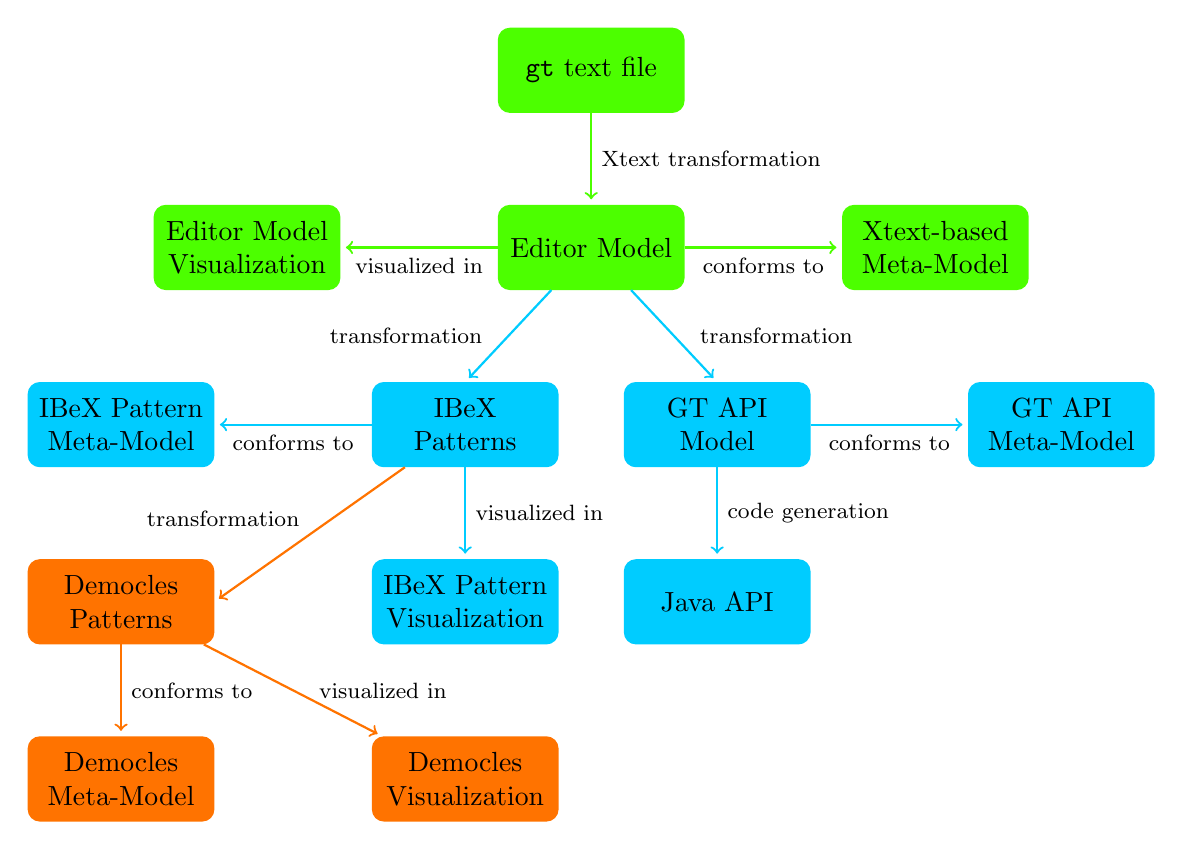
\begin{tikzpicture} [
		auto,
		node distance = 2.25cm,
		node/.style = {
			rectangle,
			rounded corners,
			thick,
			text width = 6em,
			text centered,
			minimum height = 3em,
		},
		line/.style = {
			draw,
			thick,
			->,
			shorten >=2pt,
		},
		line-caption/.style = {
			font = \footnotesize
		},
		ibex-ui/.style = {
			draw = green!60!lime,
			fill = green!60!lime,
		},
		ibex/.style = {
			draw = blue!20!cyan,
			fill = blue!20!cyan,
		},
		ibex-democles/.style = {
			draw = red!10!orange,
			fill = red!10!orange
		}
	]

	\node[node, ibex-ui] (f) {
		\texttt{gt} text file
	};

	\node[node, ibex-ui, below of = f] (e) {
		Editor Model
	};
	\node[node, ibex-ui, left = 2cm of e] (ev) {
		Editor Model Visualization
	};
	\node[node, ibex-ui, right = 2cm of e] (em) {
		Xtext-based Meta-Model
	};

	\node[node, ibex, below of = e, xshift = 1.6cm] (g) {
		GT API Model
	};
	\node[node, ibex, right = 2cm of g] (gm) {
		GT API Meta-Model
	};
	\node[node, ibex, below of = g] (gc) {
		Java API
	};

	\node[node, ibex, below of = e, xshift = -1.6cm] (i) {
		IBeX Patterns
	};
	\node[node, ibex, left = 2cm of i] (im) {
		IBeX Pattern Meta-Model
	};
	\node[node, ibex, below of = i] (iv) {
		IBeX Pattern Visualization
	};

	\node[node, ibex-democles, below of = im] (d) {
		Democles Patterns
	};
	\node[node, ibex-democles, below of = d] (dm) {
		Democles Meta-Model
	};
	\node[node, ibex-democles, below of = iv] (dv) {
		Democles Visualization
	};

	\begin{scope} [
			every path/.style = line, ibex-ui,
			every node/.style = line-caption
		]
		\path (f) -- node[right] {Xtext transformation} (e);
		\path (e) -- node[below] {visualized in} (ev);
		\path (e) -- node[below] {conforms to} (em);
	\end{scope}

	\begin{scope} [
			every path/.style = line, ibex,
			every node/.style = line-caption
		]
		\path (e) -- node[left, xshift = -0.2cm] {transformation} (i.north);
		\path (e) -- node[right, xshift = 0.2cm] {transformation} (g.north);

		\path (i) -- node[below] {conforms to} (im);
		\path (i) -- node[right] {visualized in} (iv);

		\path (g) -- node[below] {conforms to} (gm);
		\path (g) -- node[right] {code generation} (gc);
	\end{scope}

	\begin{scope} [
			every path/.style = line, ibex-democles,
			every node/.style = line-caption
		]
		\path (i) -- node[left, yshift = 0.2cm] {transformation} (d.east);
		\path (d) -- node[right] {conforms to} (dm);
		\path (d) -- node[right, xshift = 0.2cm] {visualized in} (dv);
	\end{scope}
\end{tikzpicture}

	\caption{Model transformations for eMoflon::IBeX-GT}
	\label{fig:model-transformations}
\end{figure}

To implement the features listed above, the following steps have to be completed for each feature:
\begin{enumerate}
	\item Define a textual concrete syntax and provide an editor.
	\item Provide a visualization of the editor model\footnote{\eg using PlantUML}.
	\item Define/extend an internal GT meta-model.
	\item Transform the editor model to an internal GT model.
	\item Transform the internal GT model to an IBeX pattern.\footnote{The IBeX pattern shall abstract from GT such that it can be shared with the TGG part of eMoflon::IBeX.
	In addition the IBeX pattern abstracts from different potential variants of converting a GT rule into patterns.}
	\item Provide a graphical visualization of the IBeX pattern.
	\item Transform the IBeX pattern to a Democles pattern.
	\item Design/extend the Java API.
	\item Write JUnit tests for the API using patterns/rules with the feature.
	\item Write end-user documentation (\ie add a feature description and an example in the handbook).
	\item Deploy the feature with the next eMoflon::IBeX version (for end-user testing).
\end{enumerate}

	% !TeX spellcheck = en_US
\section{Time Plan}
\label{time-plan}
Figure \ref{fig-time-plan} shows the tasks for the implementation as well as the ones for writing the thesis and preparing slides for talks with the intended weeks for their completion.

\begin{figure}[h!]
	\begin{ganttchart}[
		vgrid,
		milestone label font = \bfseries,
		milestone/.append style={draw=red, fill=red},
		bar height = 0.3,
		bar label font = \small,
		y unit chart=0.65cm
		]{1}{18}
		\gantttitlelist{1,...,18}{1} \\

		\ganttgroup{Writing Thesis}{2}{18} \\
		\ganttbar{Abstract}{2}{2} \\
		\ganttbar{Introduction}{2}{4} \\
		\ganttbar{Related Work}{4}{6} \\
		\ganttbar{Fundamentals}{7}{11} \\
		\ganttbar{Concept and Implementation}{8}{14} \\
		\ganttbar{Evaluation}{13}{16} \\
		\ganttbar{Conclusion and Future Work}{16}{16} \\
		\ganttbar{Review and Proof Reading}{17}{18} \\

		\ganttgroup{Implementation/Testing}{1}{14} \\
		\ganttbar{Simple Constraints}{1}{2} \\
		\ganttlinkedbar{Creation and Deletion}{3}{4} \\
		\ganttlinkedbar{Rule Refinement}{5}{6} \\
		\ganttlinkedbar{Attribute Conditions}{7}{9} \\
		\ganttlinkedbar{Graph Conditions}{10}{12} \\
		\ganttlinkedbar{Bugfixing}{13}{14} \\

		\ganttmilestone{Final Deadline}{18} \\
		\ganttbar{Thesis Defense}{18}{18}
	\end{ganttchart}
	\caption{Tasks, milestones and deadlines}
	\label{fig-time-plan}
\end{figure}

	% !TeX spellcheck = en_US
\chapter{Preliminary Structure}
\label{preliminary-structure}
The structure of the thesis will be similar to the following outline:

\renewcommand{\labelenumii}{\theenumii.}
\renewcommand{\theenumii}{\theenumi.\arabic{enumii}}

\renewcommand{\labelenumiii}{\theenumiii.}
\renewcommand{\theenumiii}{\theenumii.\arabic{enumiii}}

\begin{enumerate}
	\item Introduction
		\begin{enumerate}
			\item Models and Model Transformations
			\item Running Example
			\item Contribution
			\item Structure of the Paper
		\end{enumerate}
	\item Related Work
		\begin{enumerate}
			\item Features of Graph Transformation Tools
			\item Comparison of Existing Graph Transformation Tools
		\end{enumerate}
	\item Fundamentals of Graph Transformation
		\begin{enumerate}
			\item Typed Graphs
			\item Graph Conditions
			\item Rule Application
			\item Attributed Typed Graphs
		\end{enumerate}
	\item Graph Transformation with eMoflon::IBeX -- Concept and Implementation
		\begin{enumerate}
			\item eMoflon::IBeX
			\item Transformation of Graph Transformation Rules into Pattern Networks
				\begin{enumerate}
					\item Nodes and References
					\item Rule Refinement 
					\item Attribute Conditions and Assignments
					\item Graph Conditions
				\end{enumerate}
			\item Java API for Graph Transformations
				\begin{enumerate}
					\item Code Generation
					\item Usage of the API
				\end{enumerate}
		\end{enumerate}
	\item Evaluation
		\begin{enumerate}
			\item Correctness
			\item Performance
		\end{enumerate}
	\item Conclusion and Future Work
\end{enumerate}



% Bibliography
	\bibliography{../common/literature}
	\bibliographystyle{alpha}
	\label{bibliography}	
\end{document}
